\entry{Semana del 20/10/2025.} 
La idea para lo que queda de tiempo sería tratar de caracterizar el estacionario al irse prendiendo las interacciones entre tres y cuatro ondas, e intentar medir la coeficientes de interacción utilizando varios sensores (y tal vez reconstruir el espectro en el espacio $\omega-k$ usando el beamforming). 

Con el propósito de ver qué tan bien funcionaría el estacionario empecé a hacer pruebas con el código de la correlación a tres ondas para alguna de las señales que teníamos, y así determinar qué tan largas deberían ser las ventanas temporales como para llegar a ver la línea de la condición de resonancia. 

Durante ese proceso hice algunas pruebas con señales de ruido normal para ver el comportamiento del código (que debería ser lo que esperaríamos que pase al estar el motor apagado). Sin embargo, para la señal ruidosa se observa también una línea (junto a muchas réplicas) en la condición de resonancia, cuando lo natural sería que de ruido. 


\begin{figure}[!ht]
	\begin{minipage}[c]{0.5\textwidth}
			\begin{subfigure}{\textwidth}
					\centering
					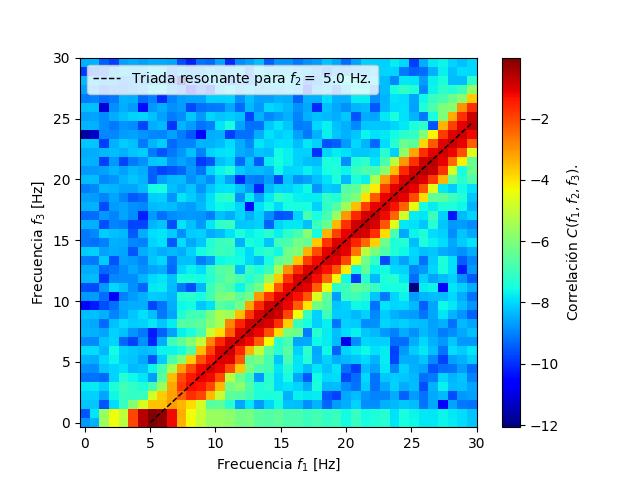
\includegraphics[width=0.8\textwidth]{Figures/20_10_2025/Señal_0_6_Hz_overlap_98_7_per.png}
					\captionsetup{width=0.8\textwidth}
					\subcaption{Señal de 0 a 6 Hz.}
				\end{subfigure}
		\end{minipage}\begin{minipage}[c]{0.49\textwidth}
			\begin{subfigure}{\textwidth}
					\centering
					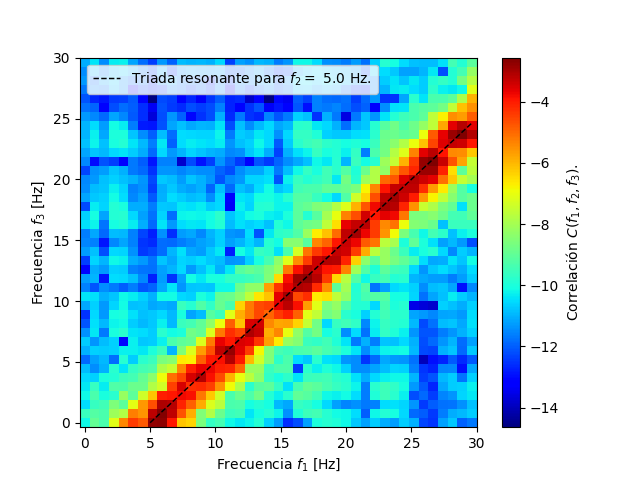
\includegraphics[width=0.8\textwidth]{Figures/20_10_2025/Señal_ruido_Hz_overlap_98_7_per.png}
					\captionsetup{width=0.8\textwidth}
					\subcaption{Ruido normal.}
				\end{subfigure}
		\end{minipage}
	\caption{Correlación de tres ondas para ruido y una señal de turbulencia de ondas con mucho overlap entre ventanas temporales (98.7\%).}
	\label{fig:triad_correlation_high_overlap}
\end{figure}

Haciendo pruebas me di cuenta que lo que generaba este artefacto en el código era usar solapamientos entre ventanas muy grandes (el conditional average dejé de usarlo por las dudas pero no cambiaba básicamente nada, y el hanning tampoco). Al bajar el solapamiento entre ventanas la correlación para el ruido daba ruido y para una señal de turbulencia de ondas la línea, como se ve más abajo. 


\begin{figure}[!ht]
	\begin{minipage}[c]{0.5\textwidth}
		\begin{subfigure}{\textwidth}
			\centering
			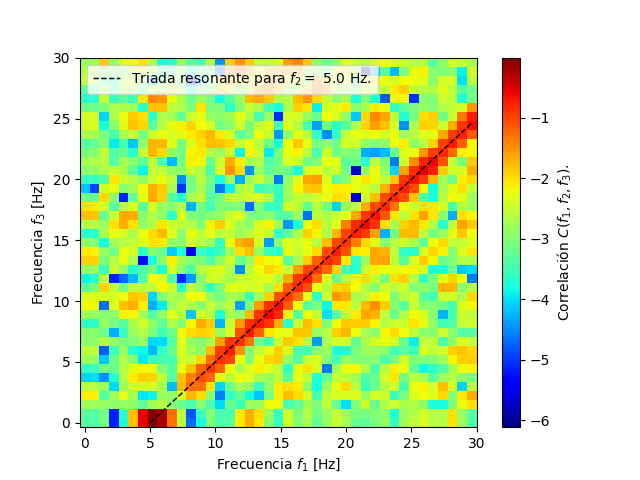
\includegraphics[width=0.8\textwidth]{Figures/20_10_2025/Señal_0_6_Hz_overlap_10_per.png}
			\captionsetup{width=0.8\textwidth}
			\subcaption{Señal de 0 a 6 Hz.}
		\end{subfigure}
	\end{minipage}\begin{minipage}[c]{0.49\textwidth}
		\begin{subfigure}{\textwidth}
			\centering
			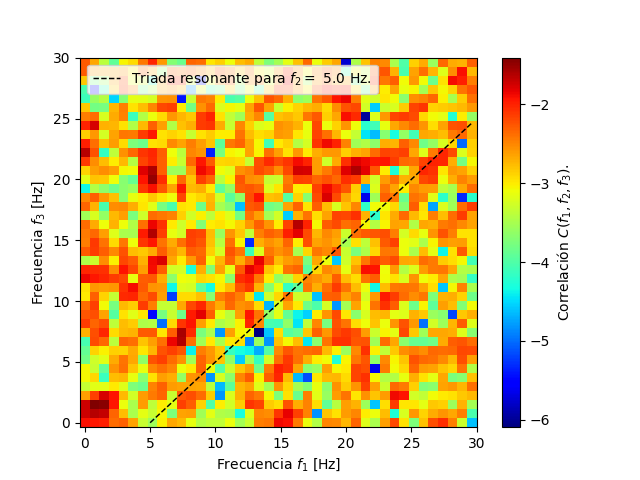
\includegraphics[width=0.8\textwidth]{Figures/20_10_2025/Señal_ruido_Hz_overlap_10_per.png}
			\captionsetup{width=0.8\textwidth}
			\subcaption{Ruido Normal.}
		\end{subfigure}
	\end{minipage}
	\caption{Correlación de tres ondas para ruido y una señal de turbulencia de ondas con poco overlap entre ventanas temporales (10\%).}
	\label{fig:triad_correlation_low_overlap}
\end{figure}


Además ahora no se ven interacciones de tres ondas para frecuencias menores a aproximadamente 10 Hz, lo cual es más pareciod a lo que observaban Aubourg y Mordant en \cite{aubourgNonlocalResonancesWeak2015}.   

Lo negativo que tiene esto es que al no poder usar superposición entre ventanas, el tiempo total de la señal debe ser mayor para tener muchos mapas que promediar. Aunque reduzcamos el tiempo de la ventana (que hace peor la resolución en frecuencia) y veamos el mapa hasta frecuencias más grandes para que se vea la línea (por ejemplo 100 Hz) igual la ventana mínima resulta de 40 segundos, con lo cual complicaría el estudio del transitorio al prender el motor. 

Un par de ideas para resolver esto serían, en lugar de ver el prendido instantáneo del motor, modular el ruido por algo que sature en 1 y crezca lentamente (tipo $1-\exp(-t\tau)$) y usar tiempos características de unos 5 minutos. Con 16000 puntos podemos llegar a señales de frecuencias máximas de unos 4 Hz que duren unos 10 minutos manteniendo buena resolución (más que eso habría que usar el input analógico que probamos antes). La otra idea de Pablo fue estudiar un solo modo e ir incorporando otro lentamente, de modo que no necesitemos calcular el mapa de correlación completo, y solo enfocarnos en esos dos.    

En adelante lo ideal sería tomar señales más largas y no tener que usar overlap durante la estadística para evitar este tipo de artefactos que todavía no tenemos muy claro de donde salen del todo. Además se pueden incluir los primeros segundos aunque esté el transitorio de la DAQ ya que no parecen modificar el resultado final en la correlación (efecto para frecuencias menores a 1 Hz aproximadamente).  